% !TEX encoding = UTF-8 Unicode

\documentclass{standalone}

% packages
\usepackage{float}
\usepackage{tabu}
\usepackage{booktabs}
\usepackage{graphicx}
\usepackage{caption}
\usepackage[export]{adjustbox}
\usepackage[utf8]{inputenc}
%\usepackage[active,pdftex,tightpage]{preview}
\usepackage{newtxtext,newtxmath}
\usepackage[percent]{overpic}

\begin{document}

%\sf
\tiny
\centering 

\begin{tabular}{m{0.5\textwidth} m{0.5\textwidth}}
%
\multicolumn{1}{c}{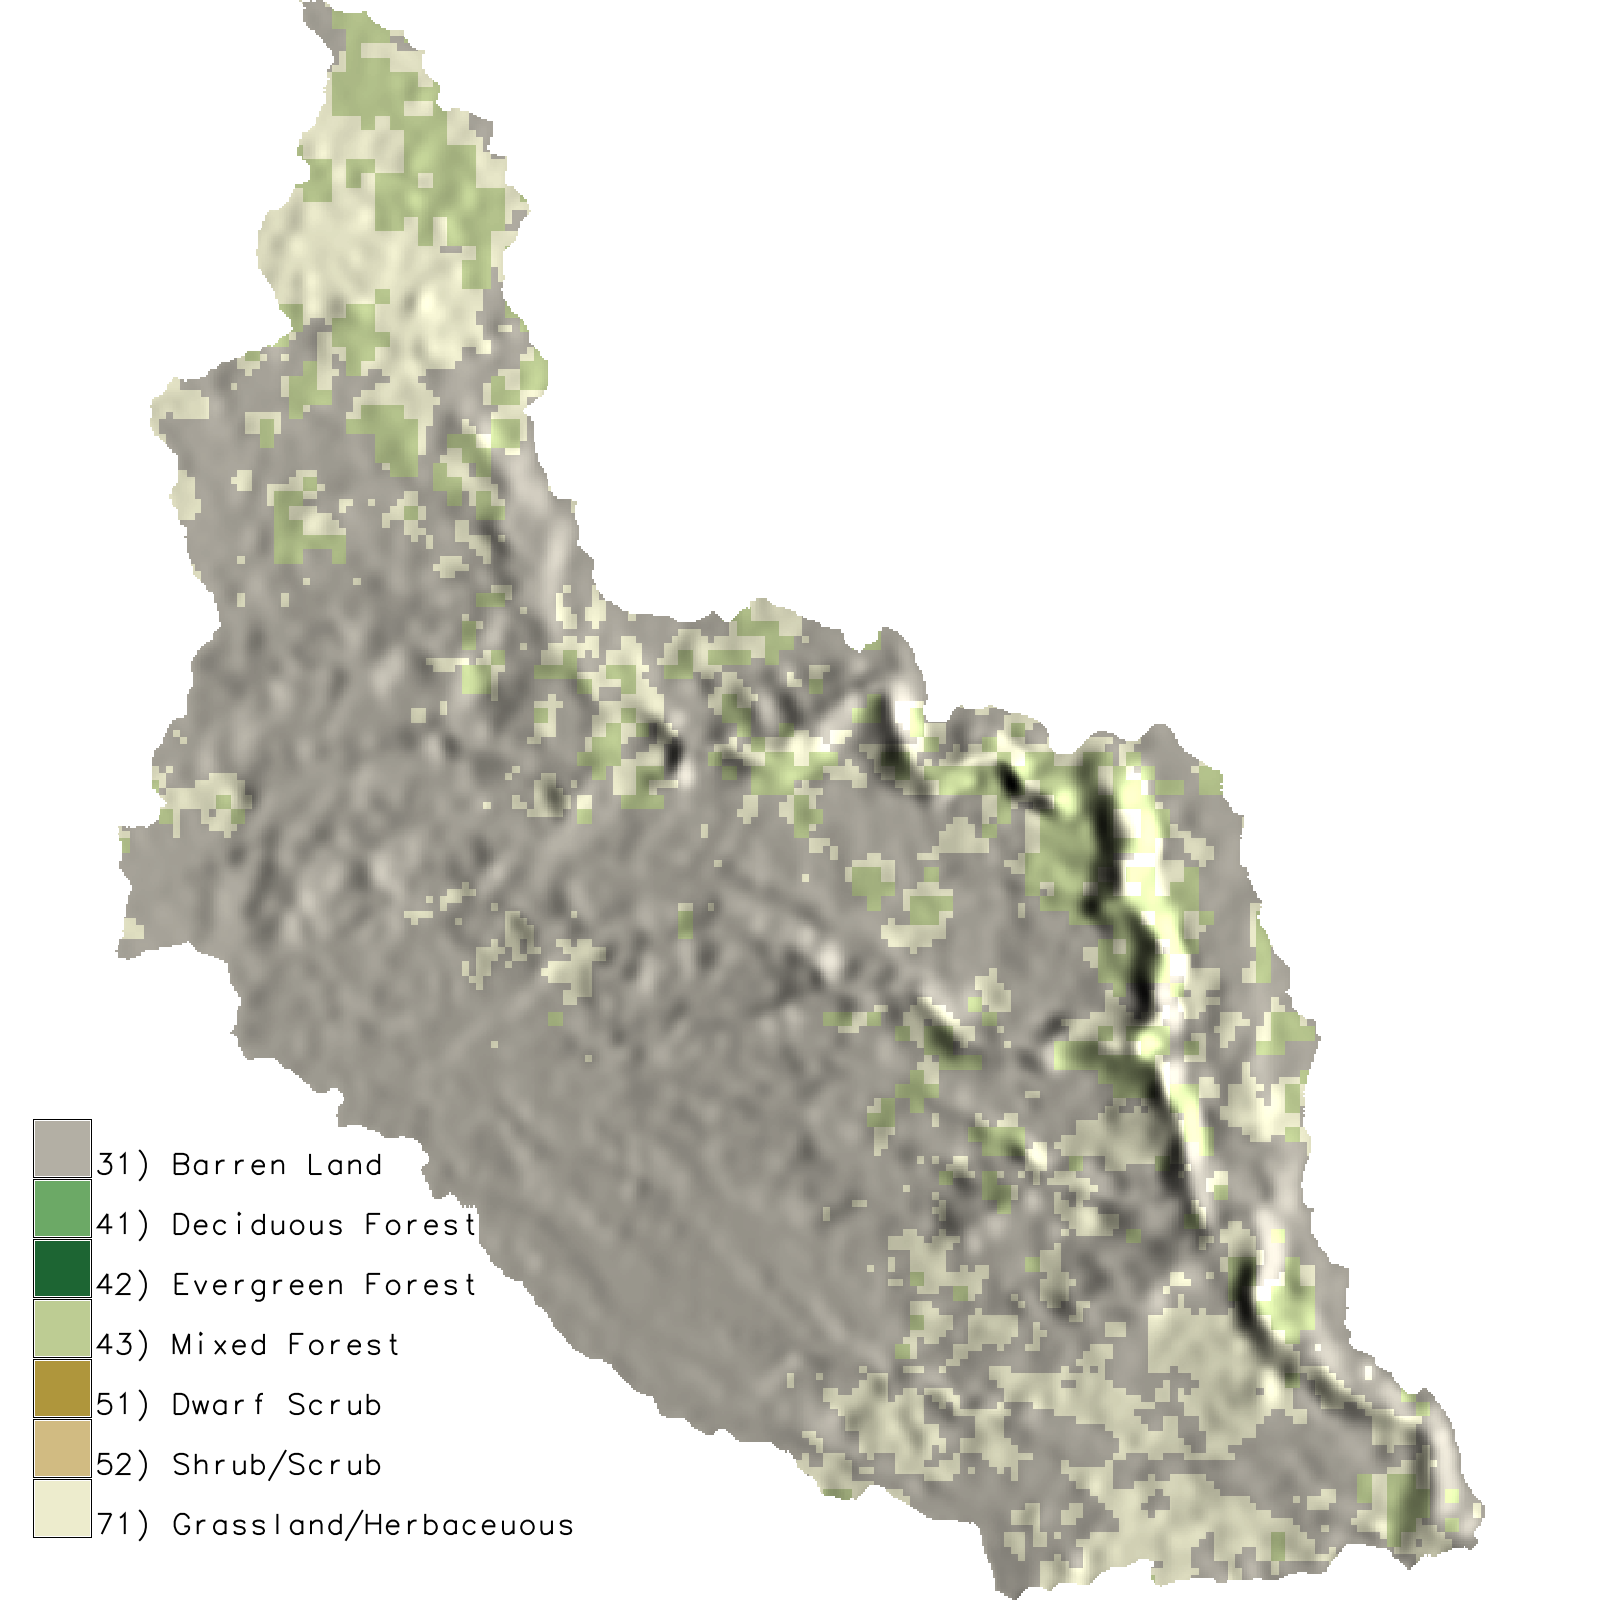
\includegraphics[height=50mm]{../../images/sample_data_detail/landcover.png}} &
\multicolumn{1}{c}{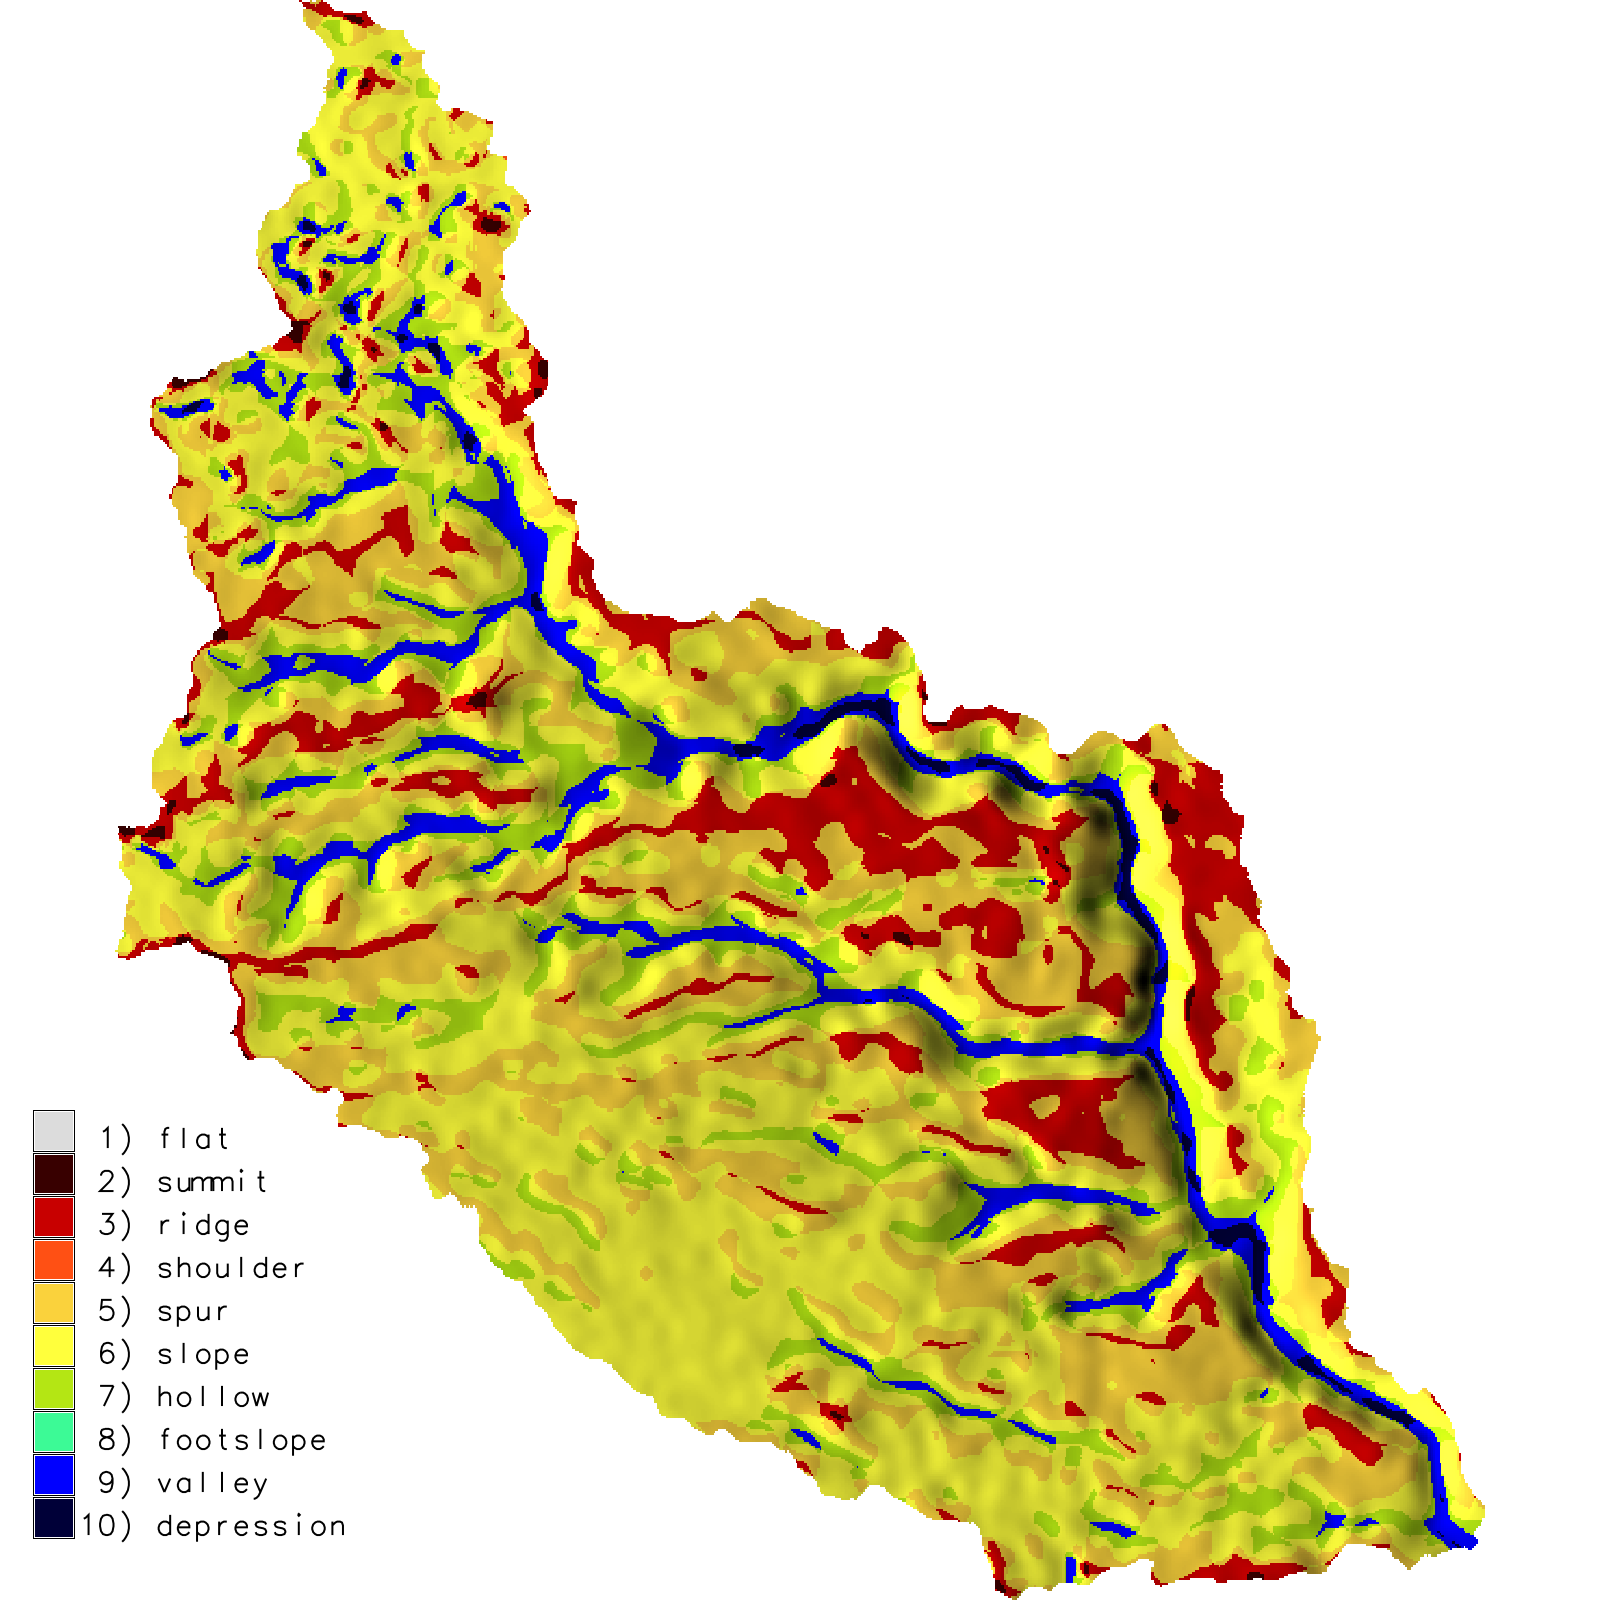
\includegraphics[height=50mm]{../../images/sample_data_detail/landforms_2012.png}}\\
\\
\multicolumn{1}{c}{a.} & \multicolumn{1}{c}{b.}\\
\\
\\
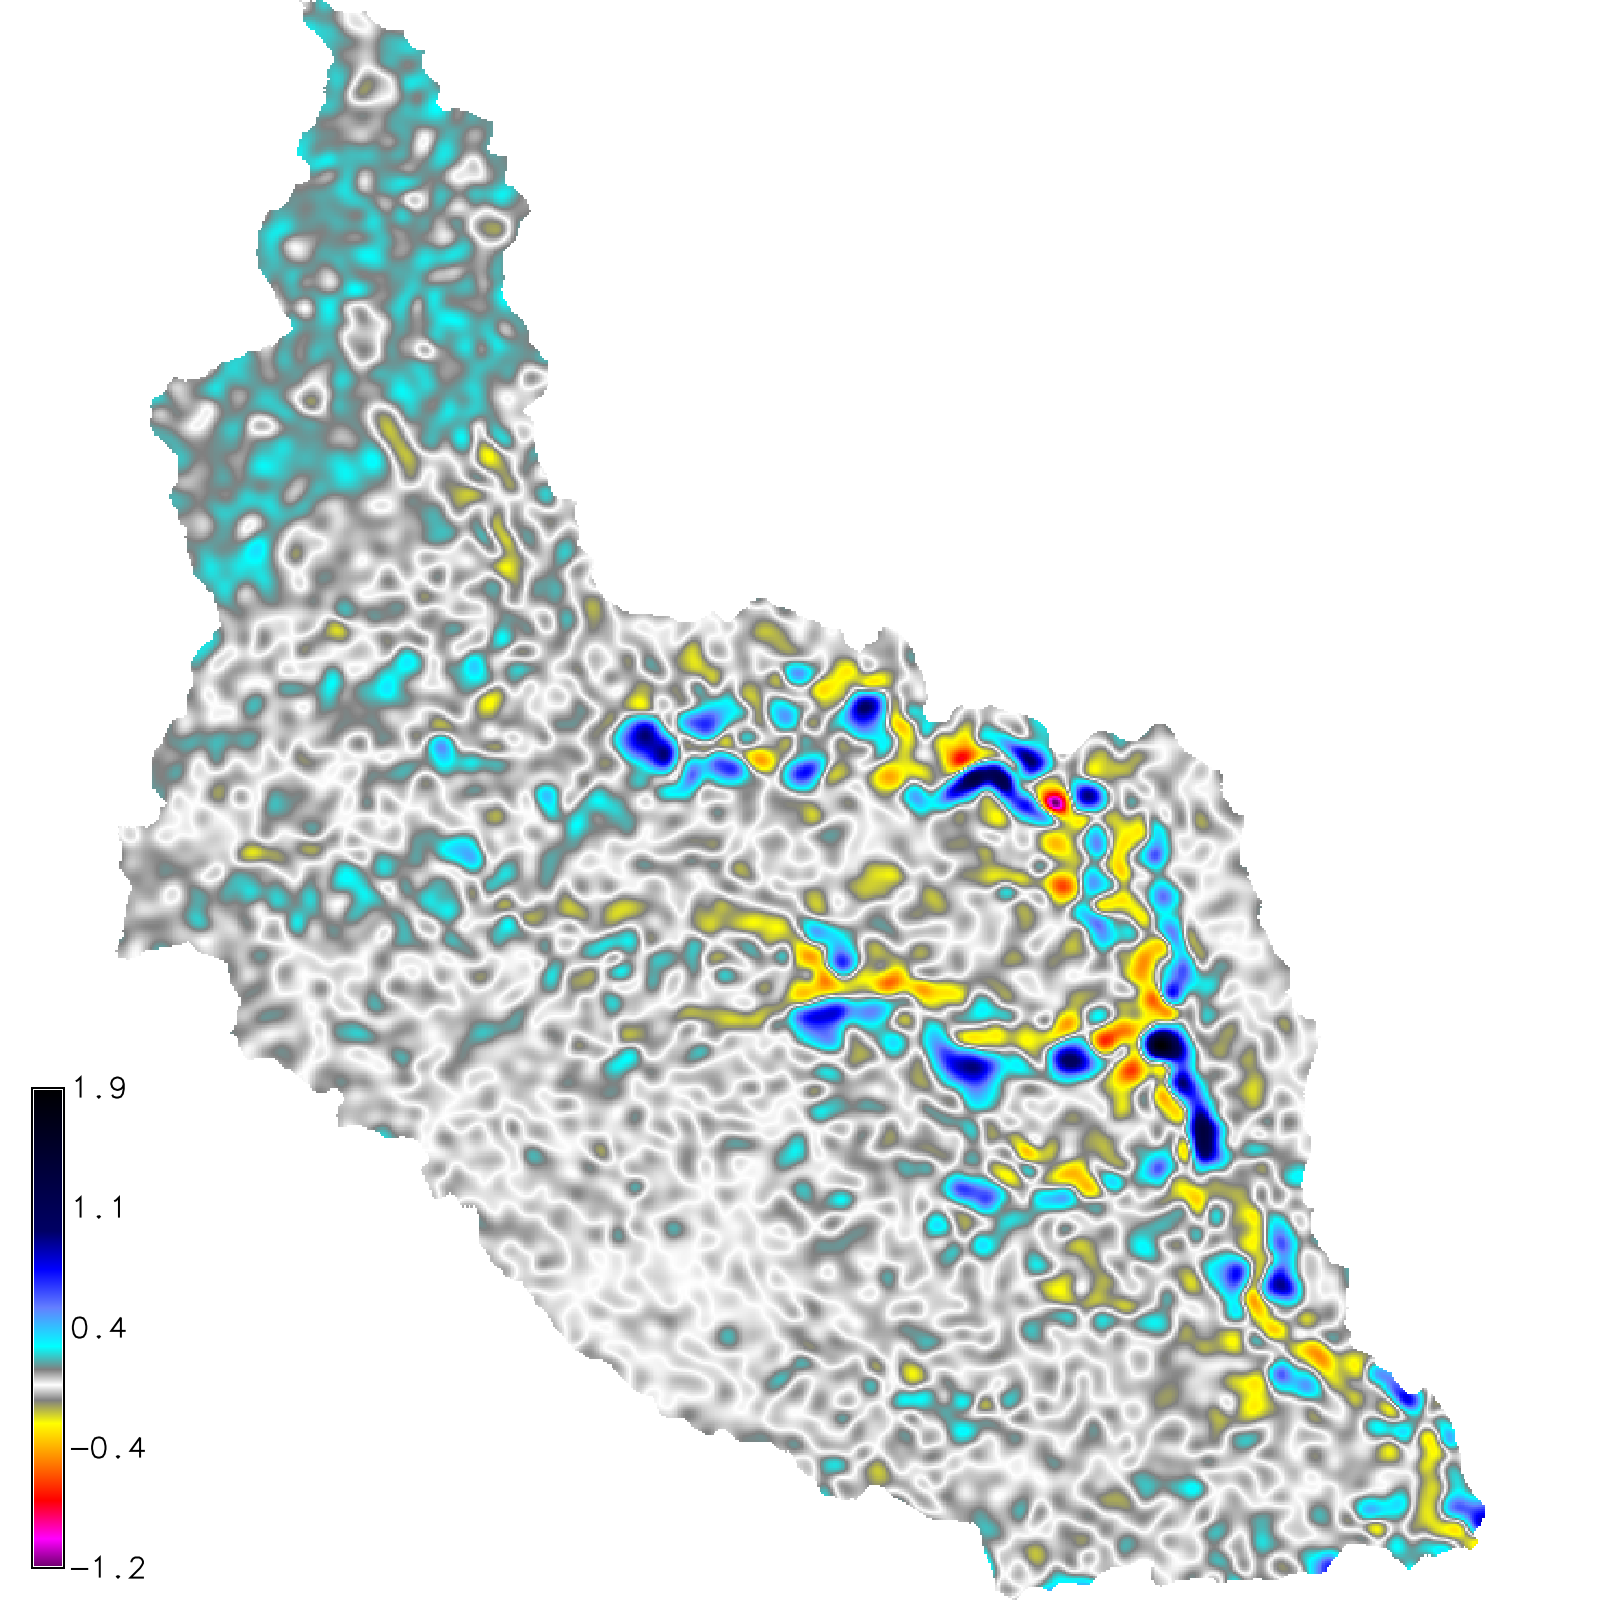
\includegraphics[height=50mm,center]{../../images/sample_data_detail/difference_2012_2016.png} &
\begin{overpic}[height=50mm,center]{../../images/sample_data_detail/landforms_2016.png}
\put(-10,-12){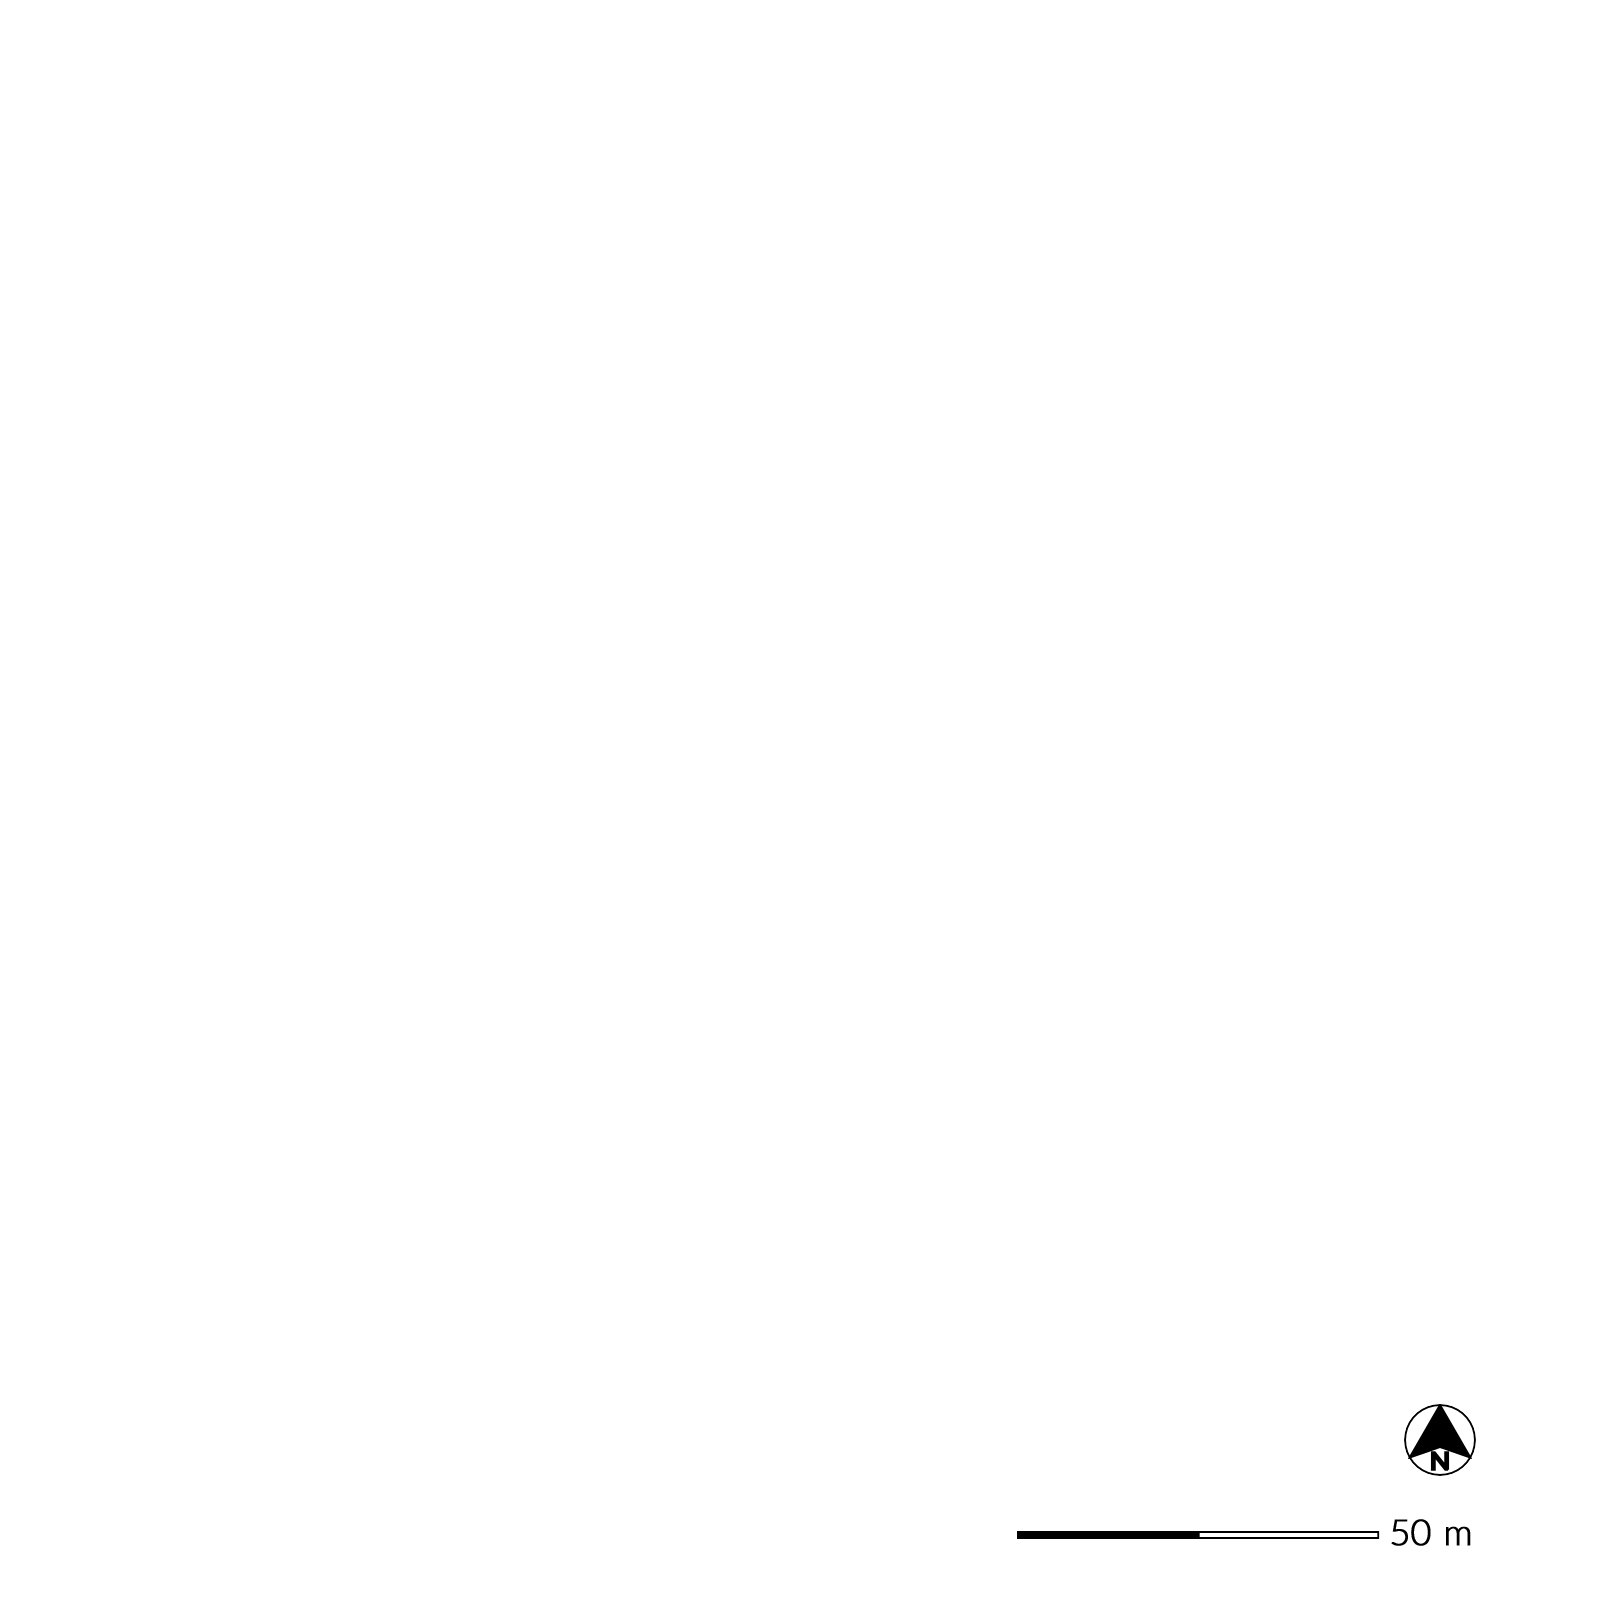
\includegraphics[height=70mm]{../../images/sample_data/map_elements_detail.png}}  
\end{overpic} \\
\\
\\
\multicolumn{1}{c}{c.} & \multicolumn{1}{c}{d.}\\
%
\end{tabular}

\end{document}

